This project is inspired by an article by \citeA{baker2009}, in which the authors modeled human goal inferences using inverse planning.
In three experiments, participants were asked to watch a short animation of what they were told was an alien moving towards a goal. In each clip, there were three goals marked in the environment, and an agent moving along a trajectory (see Figure \ref{fig:tenenbaum:env}).
The agent stopped at a point in the trajectory, which the authors call the \textit{judgement point}, and the participants were then asked to judge how likely each goal was at this point.

\begin{figure}
	\centering
	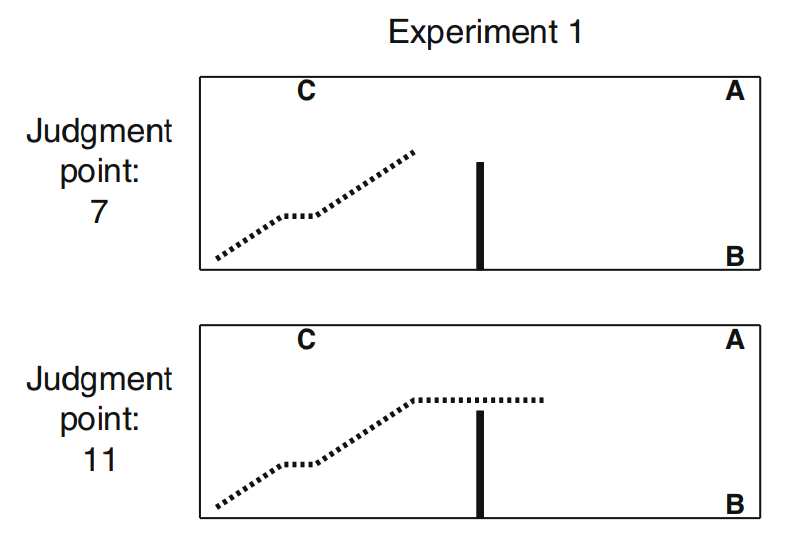
\includegraphics[width=0.7\linewidth, trim=15pt 0pt 0pt 15pt, clip]{intro/tenenbaum_exp}
	\caption{Example stimulus, from \citeA{baker2009}, Experiment 1. Participants watch a clip of what they are told is an agent moving in an environment. Three goals (A, B, C) are marked in the environment. The clip is stopped at various points in the trajectory (\textit{judgement points}), and the participants are asked to judge the probability of each goal being the goal pursued by the alien.}
	\label{fig:tenenbaum:env}
\end{figure}


The authors developed three models to solve the same task using inverse planning:
First, the environment is defined as a Markov Decision Problem for each of the goals, and the Boltzman policies are calculated. Then, with the given trajectory, the posteriors of the goals, given the trajectory, are determined. 
A more detailed account of the models will be given in \ref{subsec:models}. The authors also included a model based on a simple heuristic, as to which an agent's goal always corresponds to the one it has moved towards in the last step, thereby assessing the most likely goal continuously for each step, neglecting the history.

Lastly, the posterior goal likelihoods under each model are compared to the human participants' judgments. The authors found a good correlation between the models' predictions and the human judgments.

In this project, the modeling methods of \citeA{baker2009} will be used to create a framework with which agent movement in a 2D regular grid environment can be simulated, and, given real-life or simulated observations, inferences can be drawn to internal model parameters and structures using inverse planning.
Two types of representation are explored, the map-like regular grid representation used in \citeA{baker2009}, and a vector representation describing only distance and direction to the goals in the environment.
Moreover, the omniscient calculation process used in the original article is here contrasted with a greedy local algorithm for navigation. 

Most modeling approaches to insect navigation focus on simulating a specific skill observed in insects, such as the homing behavior in ants \cite<e.g.,>{goldschmidt2017a}, or the replication of behavior observed in specific neural circuits or areas.
Especially the insect central complex which has been connected to insect navigation \cite{honkanen2019}, is the subject of a variety of computational models \cite<e.g.,>{adden2020a,cope2017,stone2017}, which mostly focus on the topic of orientation and steering, but also on path integration.
A second neural structure that is a common target for computational modeling in the area of insect navigation is the mushroom body \cite<e.g.,>{ardin2016} to investigate insect memory.

These modeling approaches are mostly used to either replicate behavior found in in-vivo experiments, to answer questions about latent mechanisms by comparing viability of different computational approaches, or to generate new hypotheses.

This project focuses on a different question: it provides a framework for modeling approaches of trajectory-generating artificial agents.
These trajectories can then potentially be employed for the aforementioned usages of computational modeling by either asking theoretical questions, or by comparing it to real experimental data.
The inverse planning methods based on Bayesian inferences allows for freedom in the subject of researched questions and directionality and dependency of model variables.

This report is structured as follows: First, the basics of Markov Decision Problems will be explained. Second, the specific computations in the models from \citeA{baker2009} will be described.
Third, the implementation details and computations used in this project will be shown.
Fourth, three conducted experiments will be presented.
The report will be concluded with a discussion on possibilities of inverse planning for insect navigation research.